\chapter{Ground state}

\section{Polaron formation energy}


The difference between the ground state energy in the absence of electron-lattice interaction ($\lambda_{ir}=0$) and its value for the coupling value where this distortion sets in is $E_p = E(\lambda_{ir}=0)- E(\lambda_{ir}=0.13$ eV$) \sim 42$ meV and corresponds to the bipolaron binding energy. This value compares favorably with the value obtained from femtosecond time-domain spectroscopy ($E_p \sim 45$ meV for YBa$_2$Cu$_3$O$_7$ \cite{Demsar1999}. We also find that if we consider a smaller electron-lattice coupling such that the distortion is 0.08 $\AA$, as that observed for in plane Cu(2)-O in La$_{1.85}$Sr$_{0.15}$CuO$_4$ \cite{Bianconi1996}, we obtain $E_p \sim 32$ meV, which is also comparable to estimates for the pseudogap formation energy in this system \cite{Kusar2005}.

\section{Projection into phonon coordinates}

\begin{figure}[ht!]
\centering
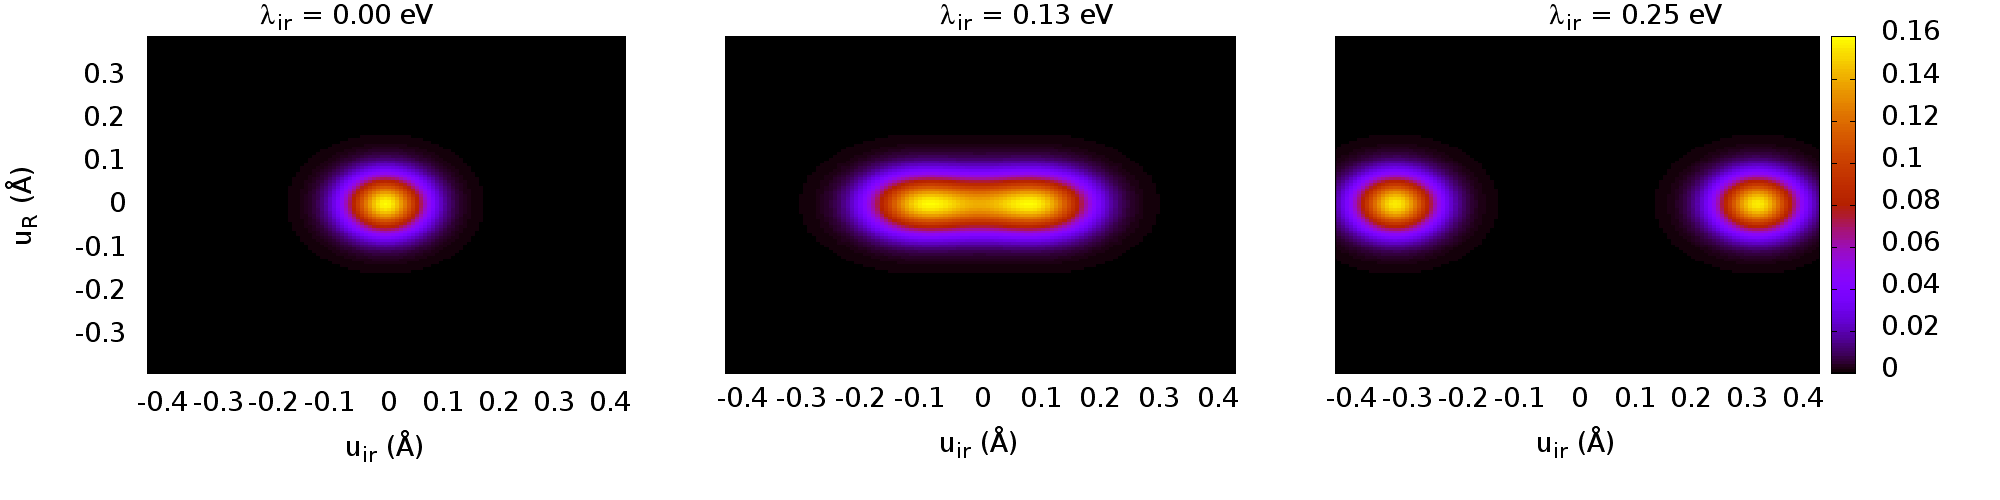
\includegraphics[width=0.8\textwidth]{images/ph-ground.png}
\caption{Ground state's projection into phonon coordinates.}
\label{fig:ph-ground}
\end{figure}

\section{Isotopic shift}

For the ground state we define the energy isotopic shift $\Delta_g$ in a similar way but with the energies measured relative to the uncoupled system (that is, the system with $\lambda_{ir}=\lambda_R=0$) (see \ref{isot-shift-def-grd}):

\begin{equation}
\Delta_g = \frac{\Delta E_g(^{16}O)- \Delta E_g(^{18}O)}{\Delta E_g(^{16}O)} \times 100 \end{equation}

where $\Delta E_g \equiv E_g - E_g(\lambda_{ir}=0, \lambda_R=0)$. To calculate this energies we need to take into account the *zero-point energy* in the phononic part $H_{ph}$ from (\ref{eq:full-hamiltonian}) writting it as \ref{phononic-part-complete}

The following figure plots this isotopic shift:

\begin{figure}[ht!]
\centering
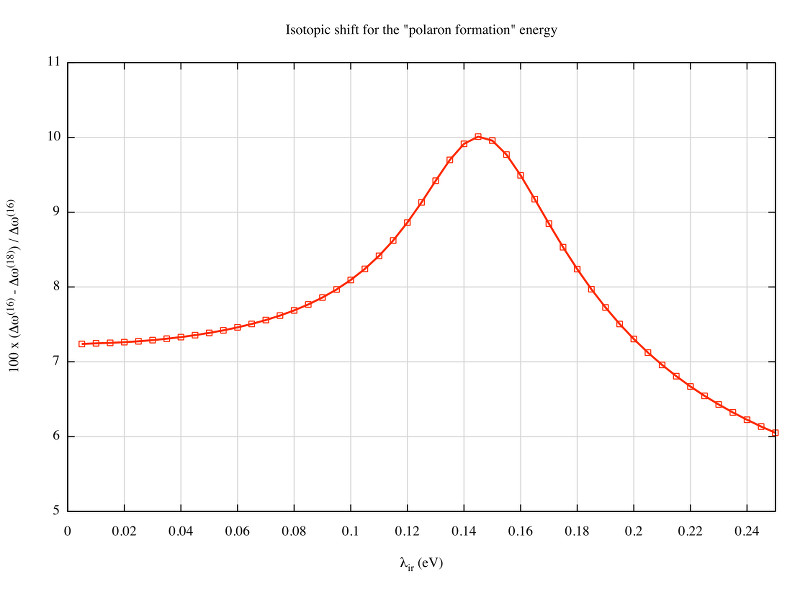
\includegraphics[width=0.8\textwidth]{images/isot_polaron_formation.jpg}
\caption{Isotopic shift of the polaron formation energy.}
\label{fig:isot_polaron_formation}
\end{figure}

Although $\Delta_g$ doesn't change sign, as the isotopic shift of the polaron tunneling state, it shows a maximum in the middle coupling regime reminiscent of the maximums, minimums or inflection points in the isotopic shifts for all the other excitations.